\chapter{Introduction}
 
The number of an observed astronomical object is often unquantifiable. A 2016 paper by \cite{conselice2016evolution} uses Hubble data to estimate the number of galaxies in the observable universe to be on the order of one trillion ($10^{12}$) out to a redshift of $z=8$. In a recent Gaia survey, 1.3 million binary stars were catalogued by \cite{el2101million}. The SIMBAD database (\cite{wenger2000simbad}) currently details over 12 million objects varying from stars, galaxies, nebulae, supernovae, and more. Its amazing that we know of millions of objects in the universe, but have only detected a few thousand exoplanets. The study of exoplanets, which are planets around other stars, is a relatively new field of science and one of the only astronomical objects we have a definite number of known detected objects. As of February $24^{th}$, 2021 (the date the author started writing her dissertation!) there are 4,352 planets according to the NASA exoplanet archive. From this limited sample we have discovered that other planetary systems look completely different from ours. The first exoplanet discovered around a sun-like star is 51 Pegasi b, a Jupiter sized planet that has an orbit closer than Mercury's to its star, (\cite{mayor1995jupiter}). 

Astronomers classify exoplanets in reference to our own solar system. The categories are based upon mass, composition and radius of the exoplanet and include but not limited to: hot and cold Jupiters, Neptunes, and super-Earths. Figure \ref{fig:exoplanets} plots the known exoplanets as a function of mass and semi-major axis of orbit relative to Earth. Different methods of exoplanet detection are indicated by different symbols. Almost all of the known exoplanets are larger than Earth, in the Neptune and Jupiter classes. This does not mean that Earth like planets are rare, but that our current techniques of exoplanet detection are biased.

\begin{figure}
    \centering
    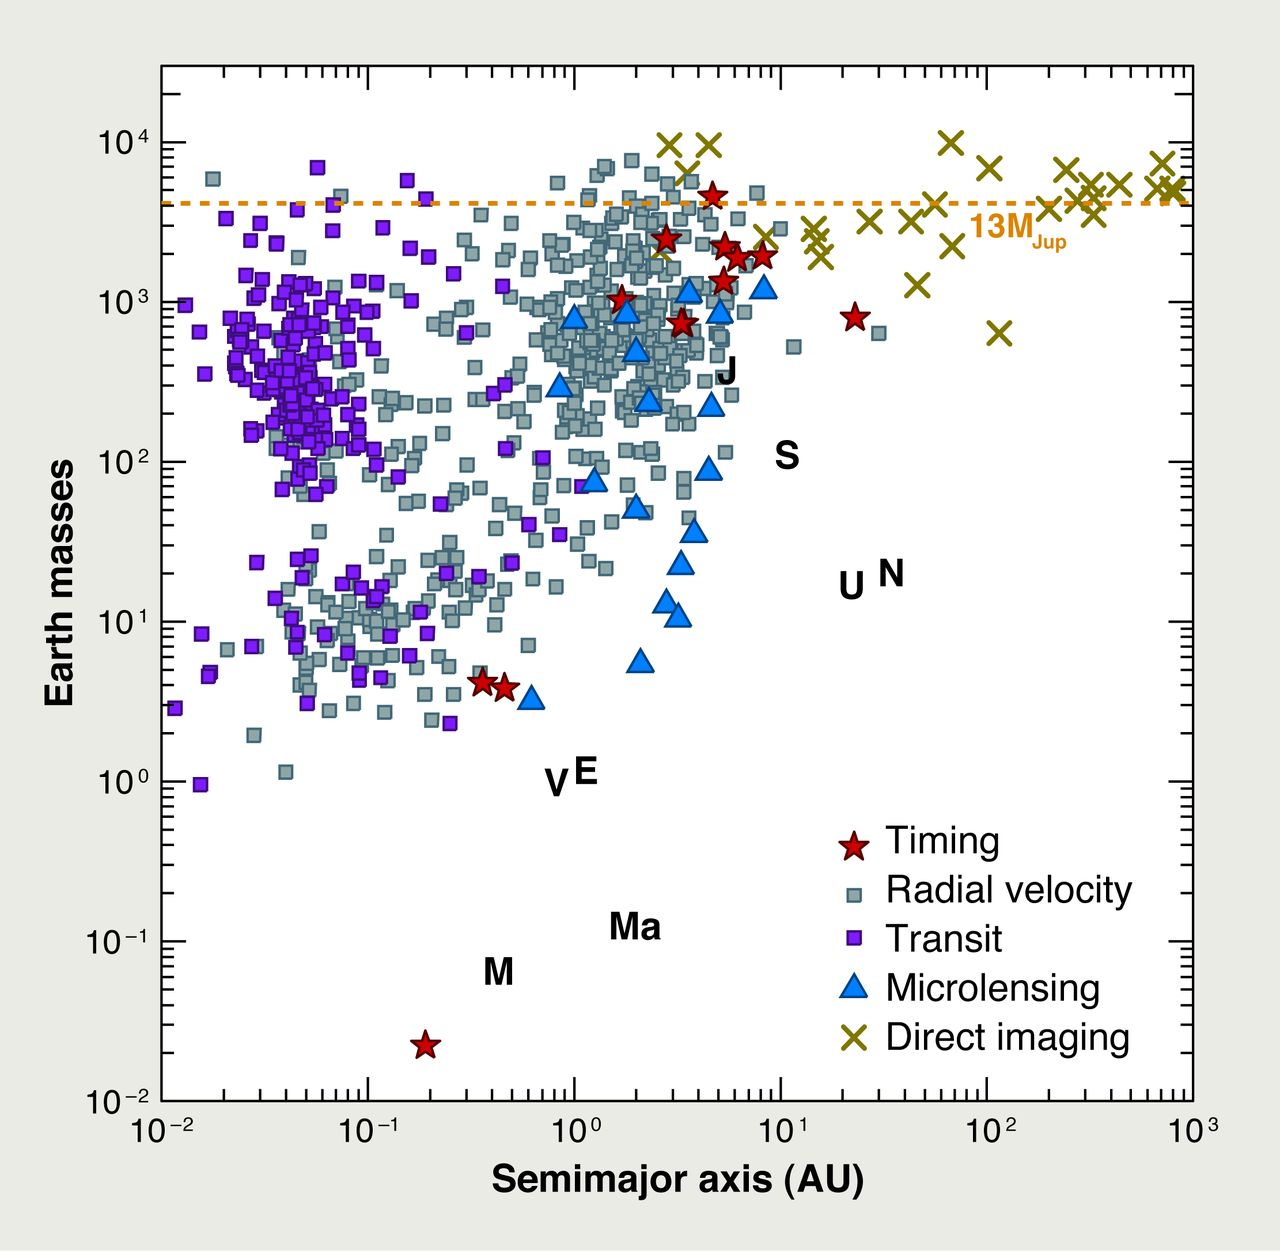
\includegraphics{Chapter Materials/Introduction Materials/Introduction Figures/F1.large.jpg}
    \caption{PLACE HOLDER FOR LOGAN'S}
    \label{fig:exoplanets}
\end{figure}

Two of the major focuses on exoplanet research are the detection, and characterization of exoplanets. Different detection techniques favor different types of exoplanets and measure different characteristics. Studying different types of planetary systems can offer insight to the formation and evolution of our own solar system. Of particular interest is the study of Earth-like planets orbiting in a region called the habitable zone. The habitable zone is defined as the region around a star where a terrestrial planet could support liquid water. The bounds of the habitable zone are determined by extremes. The inner edge is defined by the temperature where water escapes from the atmosphere due to a process called photolysis, the decomposition of molecules by light. The outer edge is defined by the formation of carbonmonoxide clouds in the atmosphere. Carbon monoxide is a poor greenhouse gas, and does not provide sufficient insulation for the planet to maintain liquid water (\cite{seager2010exoplanets}). For our own solar system the Habitable zone is around 0.95-1.37AU. An estimate of the radius of the habitable zone can be found using equation \ref{HabitableZone}, and can be solved for our own solar system by setting the temperature to T=300K, the luminosity to the solar luminosity L= 1181 $\frac{W}{m^2}$, and solving for the radius of the orbit, r. The variable $\sigma_{SB}$ is the Stefan-Boltzmann constant. 


\begin{equation}
    \sigma_{SB}T^4=\frac{L}{4\pi r^2} 
    \label{HabitableZone}
\end{equation}

The search for life and habitable words beyond our solar system is a driving force of modern astronomy and one of the most captivating questions of our time. To study exoplanets astronomers use a technique called high contrast imaging or direct imaging. In this method the planet is resolved separately from the star, allowing for a direct image of the planet to be taken as shown in Figure \ref{fig:exoplanets}, (\cite{bailey2013hd}). High contrast imaging with astrometric calibration allows an astronomer to make precise measurements of the exoplanet’s mass, period, and orbit, (\cite{seager2010exoplanets}) In combination with a spectrograph, we can directly measure the atmospheric composition of exoplanets to look for signatures of organic molecules and liquid water,(\cite{seager2015search}).   

\begin{figure}
    \centering
    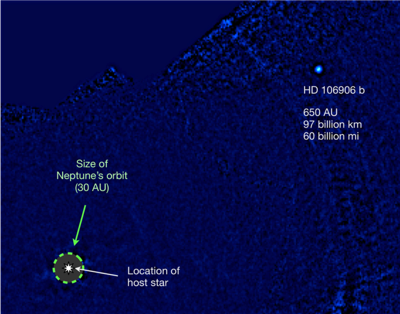
\includegraphics{Chapter Materials/Introduction Materials/Introduction Figures/HCexoplanet.png}
    \caption{Image of exoplanet HD 106906 b taken with the Magellan Adaptive Optics (MagAO) instrument. \cite{bailey2013hd}}
    \label{fig:exoplanets}
\end{figure}

Our ability to study exoplanets is limited by the high contrast problem. In direct imaging we are detecting the combination of the exoplanet’s blackbody thermal emission, and the reflected starlight off of the exoplanet’s atmosphere\cite{seager2010exoplanets} which is dwarfed by that of the host star. For example, the contrast between the Sun and the Earth is on order $10^{-10}$ in the visible spectrum. This extreme contrast ratio is the same for Earth-sized exoplanets in the habitable zone, and improves to $10^{-8}$ contrast for exoplanets around M-dwarf stars.\cite{males2014direct} Ground based observatories face additional challenges from aberrations caused by atmospheric turbulence that degrades the resolution of the image and the exoplanet can no longer be resolved.

 Overcoming this contrast problem requires a two-fold solution. The starlight needs to be suppressed by a coronagraph, and the resulting high contrast region called the dark hole needs to be maintained over the course of the observation through extreme adaptive optics (ExA0)  and wavefront sensing and control (WS$\&$C) techniques. ExAO systems operate by propagating light from a guide star to a wavefront sensor, which measures the phase error of the starlight wavefront. A computer then sends commands to shape a deformable mirror (DM) to correct for the phase error, forming a closed feedback loop that compensates for most of the atmospheric distortion. The corrected beam is then passed to a coronagraph which blocks the light from the on-axis star and allows us to detect faint off-axis companions. There are many types of coronagraphs currently used in high contrast imaging; most work by blocking out light using masks and stops\cite{soummer2004apodized}, or using interferometric techniques to destructively interfere light at the focal plane.\cite{foo2005optical} Uncorrected phase errors and  non-common path errors from the ExAO system result in speckles in the focal plane that kill coronagraph contrast. These speckles evolve with time\cite{goebel2016evolutionary} so further methods of WF$\&$C in addition to the ExAO closed loop is needed to null speckles.  

Within the next decade, the world will see a new generation of Giant Segmented Mirror Telescopes (GSMTs). The Giant Magellan Telescope\cite{fanson2020overview} (GMT) under construction at Las Campanas Observatory, Chile, will have seven 8.4-meter mirrors, forming a 24.5-meter primary mirror. The Thirty Meter Telescope\cite{chisholm2020thirty} (TMT), and the European Extremely Large Telescope\cite{ramsay2020eso} (E-ELT) at Cerro Paranal, Chile, have highly segmented primary mirrors. The 39-meter E-ELT primary mirror will be comprised of hundreds of 1.4-meter hexagonal segments. The TMT will have 492\cite{sanders2013thirty}, 1.44-meter hexagonal segments to form the 30-meter primary mirror. The GSMTs in combination with extreme adaptive optics (ExAO) systems will have the angular resolution and light collecting power to image Earth like planets around M-dwarf stars\cite{males2019gmagao}. 

Test-beds in the United States and abroad are advancing path-finding technology and techniques to enable exoplanet research on giant telescopes. One area of research is the development of different coronagraphs for telescopes that have complex apertures. There are also test-beds focused on advancing ExAO and WF$\&$C. This included techniques such as Linear Dark Field Control (LDF), Electric Field Conjugation (EFC), and Low Order Wavefront Sensing (LOWFS). Current testbeds include the High Contrast Imager for Complex Aperture Telescopes (HiCAT)\cite{2014SPIE.9143E..27N} at the Space Telescope Science Institute, the High-Contrast High-Resolution Spectroscopy for Segmented Telescopes (HCST)\cite{jovanovic2018high} test-bed at the California Institute of Technology, the Decadal Survey Testbed\cite{belikov2014ames} at the NASA Jet Propulsion Laboratory (JPL), the LAM-ONERA On-sky Pyramid Sensor test-bed (LOOPs) (CITE) at the Laboratoire d'Astrophysique de Marseille, the Occulting Mask Coronagraph\cite{shi2017dynamic} test-bed also at JPL, and the High Contrast High- Resolution Spectroscopy for Segmented telescopes Testbed (HCST) (CITE) at the California Institute of Technology. The Magellan Extreme Adaptive Optics system (MagAO-X)\cite{males2020magao} developed by the University of Arizona Extreme Wavefront Control Lab (XWCL) for the Magellan Clay Telescope, doubles as an extreme adaptive optics test-bed. Predictive real time control algorithms are being explored on MagAO-X to improve ExAO correction.\cite{haffert2021data} The MagAO-X instrument has also been involved with testing LDFC, and using a Vector Apodizing Phase Plate Coronagraph (vAPP)\cite{snik2012vector} to enable low order modal wavefront sensing.\cite{2019JATIS...5d9004M}  There are many more high-contrast imaging testbeds in existence, and many are listed on the Community of Adaptive OpTics and hIgh Contrast testbeds website.(CITE) A recent summary of current coronagraphy test-beds for space missions can be found in the decadal white paper.\cite{mazoyer2019high}


There are a number of ExAO instruments in operation on current generation telescopes. Current instruments include the Subaru Coronagraphic Extreme Adaptive Optics instrument (SCExAO)\cite{jovanovic2015subaru}, the Spectro-Polarimetric High-contrast Exoplanet Research instrument (SPHERE)\cite{beuzit2008sphere}, the Gemini Planet Imager (GPI)\cite{macintosh2014first}, the Keck Planet Imager and Characterizer (KPIC)\cite{jovanovic2019keck}, and most recently the Magellan Extreme Adaptive Optics System (MagAO-X)\cite{males2020magao}. All of these instruments have common features: a high actuator count deformable mirror running at extreme speeds (at least 1kHz), a high performance wavefront sensor (WFS), and a high-contrast coronagraph These instruments are pathfinders for ExAO systems on the GSMTs.

The GSMTs all plan to use pyramid wavefront sensors (PWFS) in ExAO instruments. The PWFS acts like a Foucault test in 2 dimensions. Light from the telescope is focused onto a glass pyramid tip where it is split and then the pupil plane is reimaged onto a detector. The result is copies of the telescope pupil that contain intensity fluctuations that are related to the wavefront phase. All current PWFS on telescopes use a four-sided pyramid (4PWFS), resulting in four pupil copies. The Planetary Systems Imager \cite{fitzgerald2019planetary} for the TMT will use a non-modulated PWFS\cite{guyon2018wavefront} in combination with lower order wavefront control to reach and maintain high contrast. The Multi-AO Imaging Camera for Deep Observations (MICADO)\cite{davies2018micado} for the E-ELT is a pathfinder instrument for performing high contrast imaging on GSMTs that uses a PWFS. The High Angular Resolution Monolithic Optical and Near-infrared Integral field spectrograph (HARMONI)\cite{neichel2016adaptive}, also for the E-ELT has a PWFS in the single conjugate adaptive optics (SCAO) mode to deliver diffraction limited performance for the E-ELT's core spectroscopic capability. The Giant Magellan Extreme Adaptive Optics System (GMagAO-X)\cite{males2019gmagao} is being developed as a first light ExAO instrument for the GMT and will use a PWFS. 

Detector size, speed, and noise all impose limits on WFS performance. The sampling of the wavefront limits the number of modes for which the adaptive optics (AO) system can correct. The read out speed of the detector sets an upper limit on the speed of the AO loop. Detector noise degrades the measurement of the wavefront error, forcing slower loop speeds to compensate, resulting in poor correction when using faint guide stars. Higher wavefront sampling requires a larger format detector which takes longer to read out. This trade-off between detector size, speed, and noise motivates the need for a new wavefront sensor architecture to build first-light ExAO instruments for the GSMTs.

(FIX THIS LAST ONE UP).


 The Extreme Wavefront Control Lab has developed the Comprehensive Adaptive Optics and Coronagraph Test Instrument (CACTI) for further experimentation in ExAO, WF$\&$C, and coronagraphy. The CACTI test-bench was designed with the flexibility to support visiting instruments and to be easily re-configurable to perform multiple experiments. In this paper we describe the design of the CACTI test-bench and the current labratory status. As an alternative to the conventional 4PWFS we are exploring a three-sided PWFS (3PWFS) as a GSMT-ExAO wavefront sensor to reduce the required number of detector pixels. The 3PWFS uses fewer detector pixels than the 4PWFS, and therefore should be less sensitive to read noise. However, the 3PWFS has not been well studied, and no 3PWFS has been tested in a closed loop adaptive optics system. The goal of this paper is to analyze the refractive three sided PWFS and demonstrate its operation in simulations. We start from the diffraction theory of the Foucault knife edge test, as the PWFS is functionally an extension of the Foucault knife edge test to two dimensions. We use the diffraction theory to motivate how we handle the signals for a 3PWFS, and test the validity in a real adaptive optics closed loop system on the LOOPS\cite{janin2019adaptive} test-bench at the Laboratoire d'Astrophysique de Marseille. Finally, we use the Object Oriented MATLAB Adaptive Optics toolbox (OOMAO)\cite{OOMAO} to simulate an end to end model of an adaptive optics system using a PWFS with modulation, and compare performance of the 3PWFS to the 4PWFS. We then discuss an experiment performed on CACTI with a visiting three-sided pyramid wavefront sensor (3PWFS) to explore an alternative wavefront sensor architecture for GSMT-ExAO. To continue this research we integrated a real 3PWFS and 4PWFS on the CACTI test-bench to test the performance of each PWFS at different levels of turbulence.







 
\section{The Telescope Signal}

The goal of an adaptive optics (AO) system is to correct for the aberrations caused by atmospheric turbulence and return the resolution of the image to the diffraction limit of the telescope. It is important to understand first what image we would expect on our detector for a perfectly corrected diffraction limited system. Noise sources, such as photon noise, affects the performance of the AO system, and influences choices on how the AO system is on-sky. In this section we will use radiative transfer and diffraction to determine what the Intensity pattern on our detector will be from a point source at infinity (a star), and an estimate of the number of photons we can expect from a star of a given magnitude. 

\subsection{Estimating the Photon Count}

We model light as an electromagnetic wave, that has a characteristic complex amplitude $A$, wavelength $\lambda$, direction $\hat{a}$, and phase $\phi$. The phase is given by $\phi= \frac{2\pi}{\lambda}*OPD$, where OPD is the optical path difference. A wave with no aberrations has an OPD=0, and the phase term disappears. Light traveling from infinity, like that of stars, is described by a plane wave in Equation \ref{waveEq}. Light spans a spectrum of wavelengths that are broken up into categories based on different proprieties of the radiation at those wavelengths. The electromagnetic spectrum spans from $10^{-12} m$ and smaller for gamma radiation, out to wavelengths of greater than $10^{-1} m$ for radio waves. Adaptive optics systems work in the visible spectrum (380nm to 700nm) out to near infrared (700nm to 5$\mu$m). 

\begin{equation}
    U=Ae^{i(k\dotr-\omega t+ \phi)}\hat{a}
    \label{waveEq}
\end{equation}

Stars exhibit black-body radiation, meaning the power spectrum of the emitted radiation has a characteristic shape determined by the temperature of the star. We can determine the expected number of photons on our telescope primary mirror from a star by integrating Plank's Law over a wavelength bandpass. Plank's Law gives the Radiant Exitance $[\frac{W}{sr*m^3}]$ of electromagnetic radiation emitted by a black-body in thermal equilibrium. We are after the energy per unit area radiated by black-body, or the Irradiance Flux Density $[\frac{W}{m^2}]$. To find the Flux Density we integrate the Radiant Exitance over a wavelength range and over the unit solid angle. The Irradiance Flux Density, $I_e$ is given by,

\begin{equation}
    I_e=\int_{0}^{2pi} d\phi \int_{0}^{\frac{\pi}{2}} \cos(\theta)\sin(\theta)d\theta \int_{\lambda_{min}}^{\lambda_{max}} \frac{2hc^2}{\lambda^5}\frac{1}{exp(\frac{hc}{\lambda k_B T})-1} d\lambda
\end{equation}

where $c$ is the speed of light, $k_B$ is the Bolzmann constant, and $h$ is Planck's constant. We have now calculated the Irradiance leaving the star, but we want to know the Irradiance arriving on Earth. To find this we do an intermediate step, by using the Irradiance Flux Density to calculate the Luminosity of the star, $L_{\star}$ [W].

\begin{equation}
    L_{\star}=I_e*4\pi r_{star}^2
\end{equation}

The Luminosity can then be used to find the Irradiance from the star at Earth, which astronomers call the Flux $F_{\Earth}$.

\begin{equation}
    F_{\Earth}=\frac{L_{\star}}{4\pi r_{\Earth}^2}
\end{equation}

Where $r_{\Earth}$ is the distance from the source to Earth. Typically in astronomy we do not need to do this full calculation to find the Flux. Stars are catalogued on an apparent magnitude scale. Equation \ref{magnitude} links the star's magnitude to the Flux, compared to a reference star of known Flux and magnitude. Vega is a common Flux zeropoint star, and there are look-up tables of flux values of Vega at different wavelength bandpasses. 

\begin{equation}
    m_1-m_2=
    2.5 \log\left(
        \frac{f_1}{f_2}
    \right)
    \label{magnitude}
\end{equation}


We now know the energy per unit area per second incident on the surface of the earth. We multiply the the Irradiance by the surface area of the primary mirror of our telescope to find Power [W], the collected energy per second.

\begin{equation}
    P=F_{\Earth}*\pi*r_T^2
\end{equation}

The estimated Energy [J] of a photon in the observed bandpass is given by,

\begin{equation}
    E=\frac{hc}{\lambda}
\end{equation}

where $\lambda$ would be the mean wavelength in the bandpass. Dividing the Power by the Energy of a photon gives the number of photons incident on our telescope per second.

\begin{equation}
    N_p=\frac{P}{E}
\end{equation}

This is an ideal estimate, as it assumes all photons from the star in that bandpass reach the the instrument. The actual Flux incident on the telescope includes factors to account for the transmission of Earth's atmosphere, transmission of all the optical components in the system, and the efficiencies of reflecting optics including that of the telescope primary and secondary mirrors. 

\subsection{Photon Noise}

In the previous section we figured out how to estimate the average photons per second we expect from a star of a given magnitude. The counting of photons is a random process described by the Poisson distribution. The error on our measurement of photon count is called Photon Noise and is the dominant error in a pyramid wavefront sensor error budget. Suppose we are counting photons over a time $T$, in discrete intervals $dt$. The photon rate of emission by the source is $v$, in units of photons/second. The average number of photons counted is $<m>=T/dt * vdt=Tv$. The probability of counting $m$ number of photons in the time interval $T$ is therefore,
\begin{equation}
    P(x)=\frac{e^{-Tv} (Tv)^m}{m!}
\end{equation}
which is the Poisson distribution. The variance of values in the Poisson distribution is $\sigma^2=m$, and the standard deviation is $\sigma=\sqrt{m}$. 

In a pyramid wavefront sensor we measure the wavefront error using Intensity on a detector. As the number of photons incident on the detector increases, the Poisson distribution approaches a Normal distribution via the central limit theorem. The noise on a measurement from a Poisson distribution is the square root of the total number of photons counted, $\sigma_I=\sqrt{N}.$ This uncertainty in our photon count directly corresponds to an uncertainty in the measurement of the shape and amplitude of the wavefront aberration. In the linear regime we expect the statistics of measured wavefront error to follow the Poisson distribution as well because we are measuring wavefront error using Intensity measurements. For each wavefront sensor there is a direct relation between the photon noise and the error on the wavefront measurement, and we quantify it through the value $\beta_p $, \cite{guyon2005}.

\subsection{The Point Spread Function}

Returning to our definition of light as an electromagnetic wave we can predict the propagation of light through our system and ultimately the distribution of light on the focal plane through diffraction. To start we assume a plane wave, as in equation \ref{waveEq}. To propagate the wave through our telescope aperture and accurately predict the intensity distribution in our focal plane we use diffractive optics. Geometric optics describes the propagation of light as rays, and assumes one point in the object is mapped to one point in the image. In geometric optics a perfect point source object would form a perfect point image. In reality, the size of an imaged point source is finite and determined by the diffraction of light from the size, shape, and power in the aperture of our system. Diffractive optics assumes that each point in the object emits a spherical wave, and the pattern at the observation point is determined by the interference of each of those wavelets. There are approximations to the diffractive theory, and in this section we assume the Fraunhofer approximation, which assumes the plane of observation is far from the plane of diffraction ($a^2 << \lambda z$ , a= radius of aperture), and that there is a limiting aperture in the pupil plane of the optical system. The Fraunhofer equation to find a field $U_z$ given a starting field $U_0$ with aperture function $T_{a}$ is given by equation \ref{Fraunhofer}.

\begin{equation}
U_z=\frac{e^{ikz}}{ikz}e^{i\frac{\pi (x^2+y^2)}{\lambda z}}\int_{\infty} U_0(\xi,\zeta)T_{ap}e^{\frac{-2\pi i(x\xi+y\zeta)}{\lambda z}}d\xi d\zeta
\label{Fraunhofer}
\end{equation}

The values $\xi$ and $\zeta$ are the spatial frequencies associated with the spatial coordinates x and y. The Fraunhofer diffraction equations calculates the Fourier Transform of the field times the aperture function.

A light wave consists of oscillating electric and magnetic fields. In diffraction theory we consider the propagation and diffraction of the electric field component, and refer to it simply as 'the field'. The methodology of solving diffraction problems is to start with a source, propagate the wavefront from the source to the plane of diffraction to find $U^-$, the field just before the aperture. We then solve for $U^+$ the field after the aperture, and then apply Fraunhofer diffraction to find $U_z$, the field at the observation plane some far distance $z$ from the aperture. If the source is a perfect point source the field at the focal plane of the image system is defined as the Point Spread Function (PSF).

To start we assume that a star is far enough away to be considered a point source. Point sources emit spherical waves, but the propagation distance from a star to the earth is far enough away that the incident wave is a plane wave. The telescope aperture is the diffractive plane in the system and can be modeled as a circular binary mask in the simplest case. After we then propagate the light to the focal plane. A diagram of this problem is given in Figure \ref{fig:propagation}. 

\begin{figure}
    \centering
    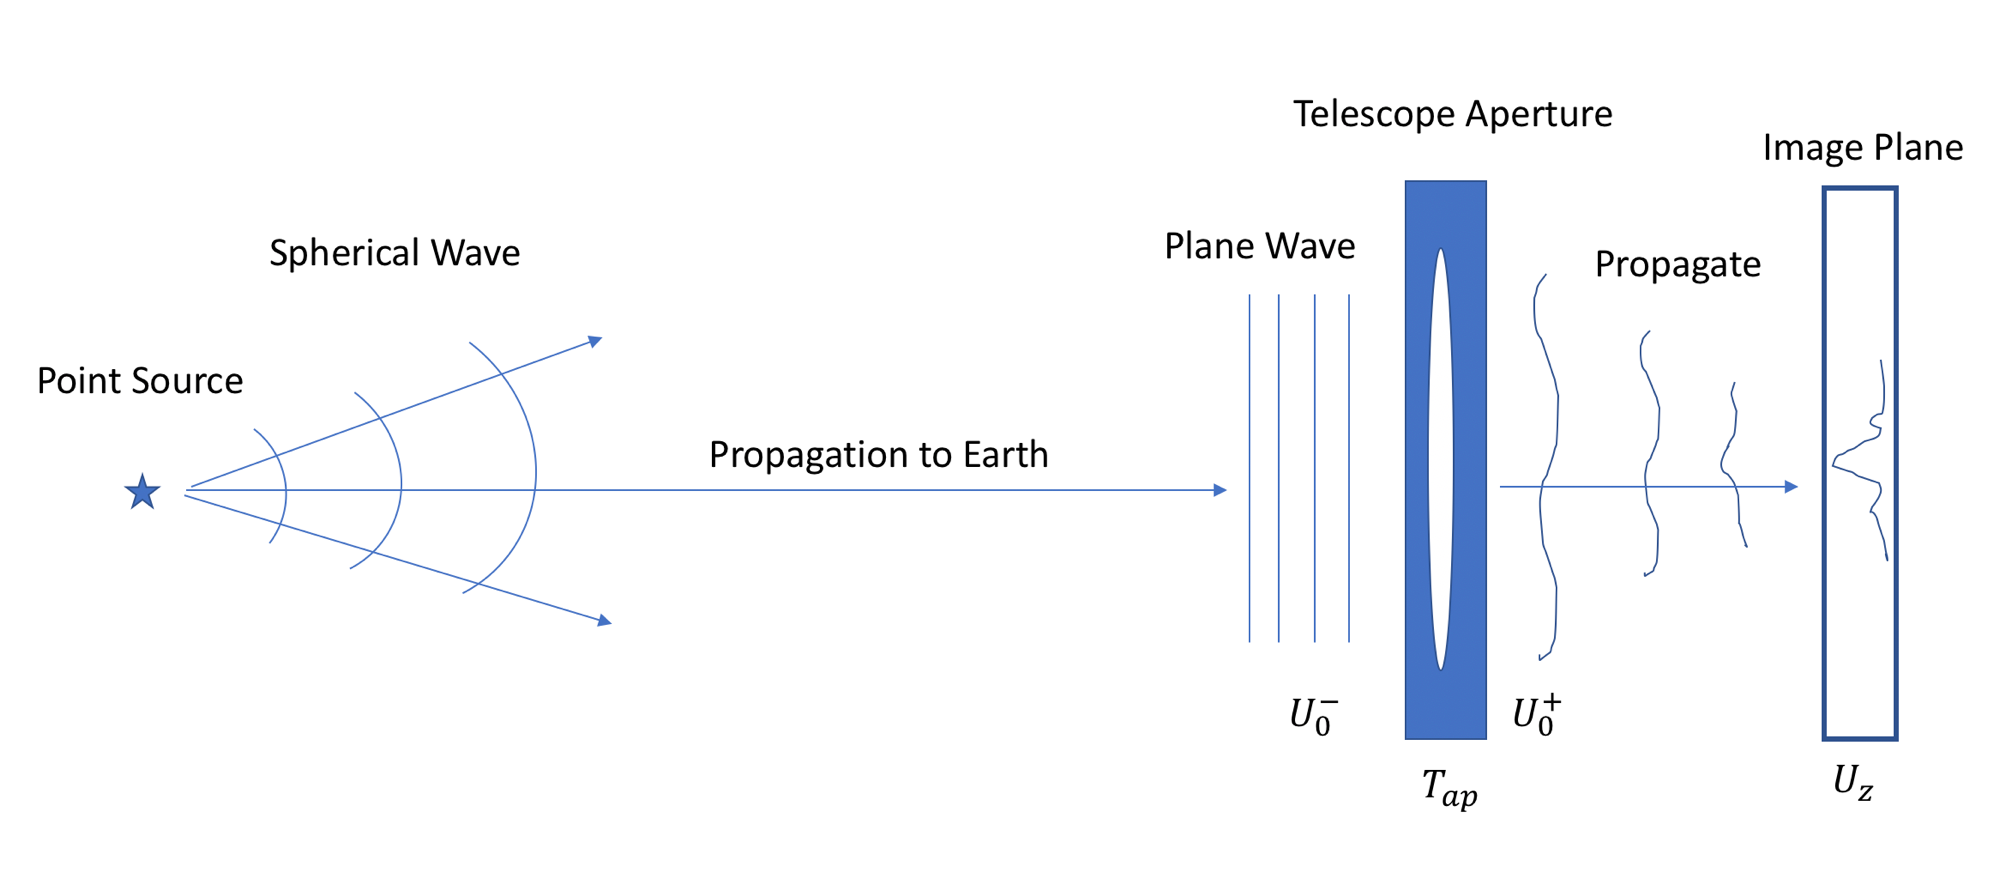
\includegraphics[width=0.75\textwidth]{Chapter Materials/Introduction Materials/Introduction Figures/Propagation.png}
    \caption{Caption}
    \label{fig:propagation}
\end{figure}

In this setup a $U_0^-$ is a perfect plane wave, that is $U=Ae^{i\phi}$ where A=1, $\phi =0$, so $U_0^-=1$. The point spread function is then just the Fourier Transform of the aperture function. The aperture function of a telescope is modeled by a circle function with diameter D, $circ(\frac{\sqrt{x^2+y^2}}{D})$, which by has a known Fourier transform that can be solved for by defining $r=\sqrt{x^2+y^2}$ and $\rho=\frac{r}{\lambda z}$. The Fourier Transform of a circ function is:

\begin{equation}
    FT(circ(\frac{r}{D/2}))=\pi{(\frac{D}{2})}^2 \frac{J_1(\pi D \rho)}{\frac{D\rho}{2}}
\end{equation}

which is a sombrero function. The Fraunhofer diffraction of a plane wave through a circular aperture is thus, 

\begin{equation}
   U_z=A\frac{e^{ikz}}{ikz}e^{i\frac{\pi (r^2)}{\lambda z}}\int_{\infty} Circ(\frac{r}{D/2})e^{\frac{-2\pi i (r \rho )}{\lambda z}}rdrd\phi= \frac{e^{ikz}}{ikz}e^{i\frac{\pi (r^2)}{\lambda z}} {\pi(\frac{D}{2})}^2 \frac{J_1 (\frac{\pi Dr}{\lambda z})}{\frac{Dr}{2\lambda z}}
\end{equation}

or,

\begin{equation}
    U_z=A\frac{e^{ikz}}{ikz}e^{i\frac{\pi (r^2)}{\lambda z}} {\pi(\frac{D}{2})}^2 somb(\frac{2r}{\lambda z})
\end{equation} 

The intensity is the modulus squared of the field,

\begin{equation}
    I(r)=A^2{\pi^2(\frac{D}{2})}^4 somb^2(\frac{2r}{\lambda z})
\end{equation}

which is the Airy pattern. For more complicated apertures the PSF can be calculated easily in simulation by modeling the aperture as a binary mask, and taking the 2D Fourier transform. The simulation can also include the predictions from section 1.1 by setting the sum of the intensity over the PSF image to the estimated number of photons. Figure \ref{fig:Airy} shows simulated PSF for a circular aperture, and the entrance pupil of the GMT.

\begin{figure}
    \centering
    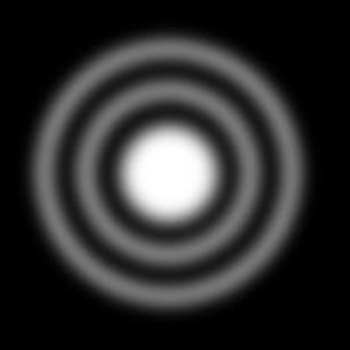
\includegraphics[width=0.5\textwidth]{Chapter Materials/Introduction Materials/Introduction Figures/Airy_disk_Placeholder.jpg}
    \caption{PLACE HOLDER}
    \label{fig:Airy}
\end{figure}


The PSF constrains the resolution of the system. For an Airy pattern the angular resolution is,

\begin{equation}
    \theta=\frac{ \lambda}{D}
\end{equation}
Two objects are considered resolved if they are at least $\frac{ \lambda}{D}$ in separation. To find the physical spot size on a detector we multiply by the effective focal length of the optics forming the focal plane.

\begin{equation}
S=\frac{ \lambda F}{D} = \lambda F_\#
\end{equation}

\subsection{Aberrations}

The resolution of a system is degraded by aberrations in the phase of the light wavefront. They arise from sources like imperfect manufacturing of optics, misalignment in the optical system, and turbulence from the atmosphere. Aberrations are described by the Optical Path Difference (OPD) the deviation of the wavefront from a perfect reference which is illustrated in Figure \ref{fig:OPD}. OPD is measured in units of length, and is related to the wavefront error [radians] by $WFE=\frac{2\pi OPD}{\lambda}$. The OPD can be a complicated function, so we often describe the aberrations as a summation of modes in a basis set. A common basis set are Zernike polynomials, which are particularly useful because the first 15 Zernike polynomials describe errors from system misalignment and are orthogonal over a unit circle. 

\begin{figure}
    \centering
    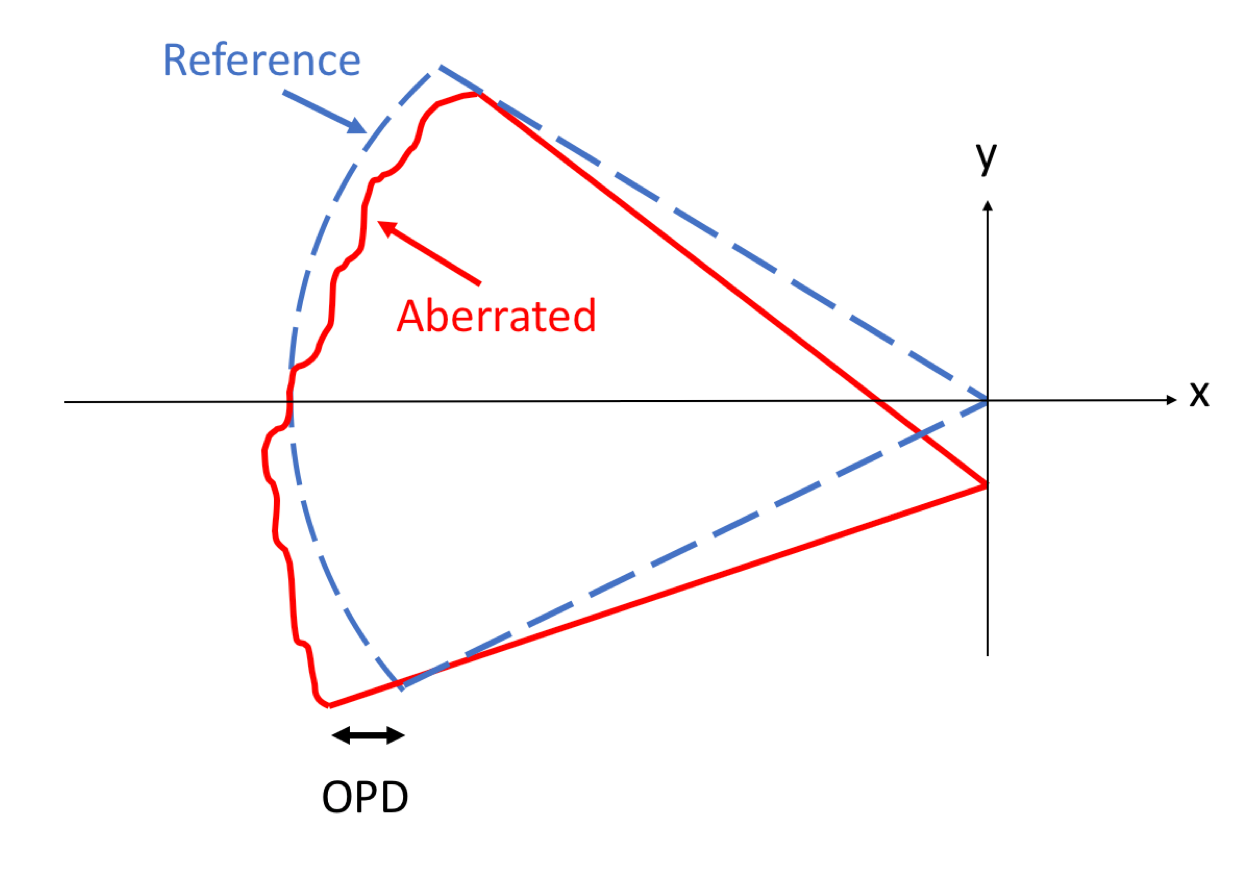
\includegraphics[width=0.75\textwidth]{Chapter Materials/Introduction Materials/Introduction Figures/OPD.png}
    \caption{Caption}
    \label{fig:OPD}
\end{figure}

The Zernike Polynomial generating function is,

\begin{equation}
    \begin{split}
        U_n^m(\rho,\phi)_{even}=R_n^m(\rho)cos(m\phi) \\
        U_n^m(\rho,\phi)_{odd}=R_n^m(\rho)sine(m\phi)
    \end{split}
\end{equation}

where $R_n^m(\rho)$ is,

\[ 
R_n^m(\rho)= \left\{
\begin{array}{cr}
       {\sum_{l=0}^{(n-m)/2} \frac{(-1)^l(n-l)!}{l!(\frac{1}{2}(n+m)-l)!(\frac{1}{2}(n-m)-l)!}\rho^{n-2l}} &  \mbox{for n-m even} \\
        {0} &  \mbox{for n-m odd} \\
\end{array} 
\right. 
\]

and $\rho$ and $\phi$ are the radial and azimuthal coordinates, (\cite{weisstein2002zernike}). The first few Zernike polynomials are given in Figure \ref{fig:zernikes}. To simulate a phase aberration, a summation of Zernike polynomials weighted by amplitude of the aberration are added into the pupil plane as a phase error. The resulting PSF is distorted due to the wavefront error, and the resolution of the optical system is degraded. An example of this is shown in Figure \ref{fig:zernikePSFs}.

\begin{figure}[h]
    \centering
    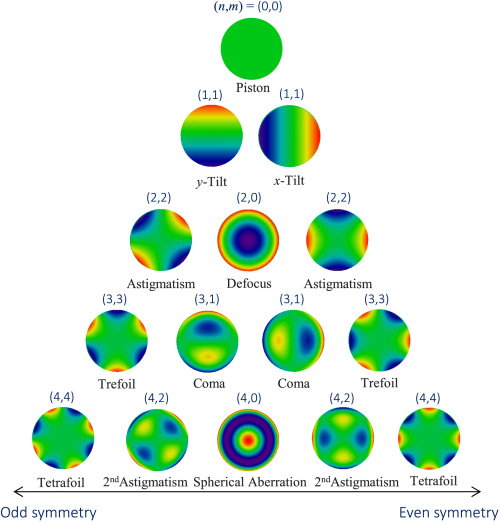
\includegraphics[width=0.5\textwidth]{Chapter Materials/Introduction Materials/Introduction Figures/zernikes.jpeg}
    \caption{First 15 Zernike polynomials. \cite{Hsieh:20}}
    \label{fig:zernikes}
\end{figure}


\begin{figure}
    \centering
    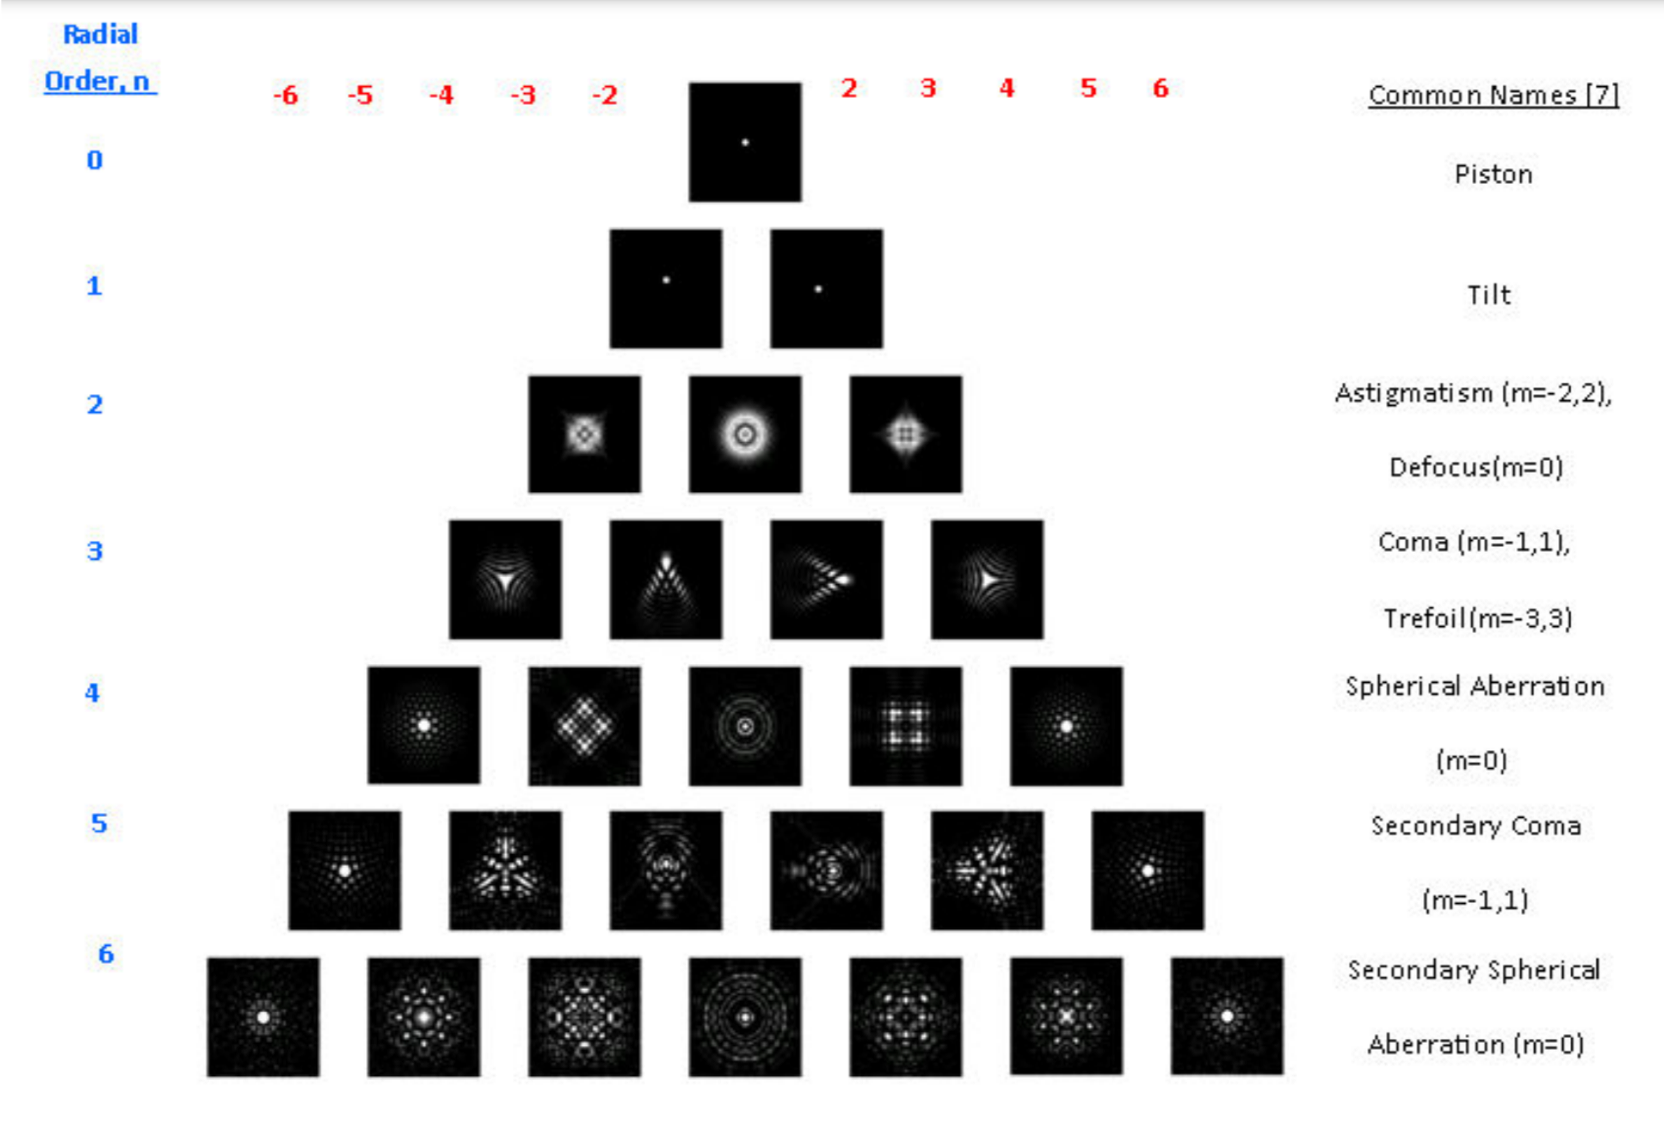
\includegraphics[width=0.75\textwidth]{Chapter Materials/Introduction Materials/Introduction Figures/ZernikePSFs.png}
    \caption{PSFS for different Zernike modal wavefront errors. \cite{masalehdan2010modeling}}
    \label{fig:zernikePSFs}
\end{figure}

\section{Atmospheric Turbulence}
In the previous sections we have learned how to calculate the flux of a star based on temperature, and use this to calculate the contrast of a star-planet system. We then propagated the light to our telescope on Earth. Now we need to take in the phase effects from propagating through Earth’s atmosphere. 

To start Earth’s atmosphere is made up of layers that have different temperatures. At the boundary between two layers, the temperature gradient causes a shearing effect that results in turbulence. The tropopause (height ~10km) contributes the largest effect of turbulence on image quality. Typically we talk about the effect of turbulence using the Kolmogorov turbulence model. In this model the turbulence imparts phase errors through turbulent eddies. These eddies dissipate heat by breaking into smaller and smaller turbulent cells. Each of these cells has a slightly different index of refraction, and the inhomogeneities in refractive index impart phase errors on the wavefront. The turbulence power spectrum is therefore defined by an outer scale $L_0$ and an inner scale $r_0$. The term $r_0$ is the Fried parameter, and it is defined as the coherence length at which the wavefront error over a circle of radius $r_0$ is 1 radian, (\cite{roddier1999adaptive}).  Each of these cells have their own index of refraction, and impart phase errors in the propagating wavefront. 

Turbulence is a statistical process we are interested in determining the evolution of refractive index at a point $x$ and another point $\Vec{r}$ away. The variance of the difference between the values at these two points is the structure function. The structure function of refractive index is given by the variance of the refractive index at points $x$ and $x+r$. 

\begin{equation}
    D_N(r)=<|N(x)-N(x,r)|^2>=C_N^2r^{\frac{2}{3}}
\end{equation}

The value of $C_N^2$ is determined through an atmospheric model that factors in the height and pressure at different atmospheric layers. This equation is only valid if the separation between the two points is less than the outer scale of the turbulent eddy.  Now we want to describe the temporal evolution of the structure function at a point $x$. The structure function is used to determine $r_0$.

\begin{equation}
    r_0=[(\frac{2\pi}{\lambda})^2 \int_0^{L_T} C_N^2(z)dz]^{\frac{-3}{5}}
\end{equation}
 
 Where $L_T$ is the total path length of the observation. The seeing $\epsilon$, is a metric used to describe the amount of blurring caused by turbulence at a given wavelength.
 
 \begin{equation}
     \epsilon=\frac{\lambda}{r_0}
 \end{equation}
 
 The mean square wavefront error over a telescope aperture of diameter D due to atmospheric turbulence is calculated using $r_0$.
 
 \begin{equation}
     \sigma^2=1.03(\frac{D}{r_0})^{\frac{5}{3}}
 \end{equation}

The Fried parameter has some useful scaling properties as well, $r_0 \propto \lambda^{\frac{6}{5}}$, and $r_0 \propto AirMass^{\frac{-5}{3}}$.

The effect of atmospheric turbulence is to lower the resolution of the optical system. For a long exposure image the image is a disk with a resolution of $\approx \frac{\lambda}{r_0 }$. For short exposure images we expect a speckle pattern of approximately $\frac{D}{r_0}$ speckles of width equal to the diffraction limit of the system. For a system partially corrected for by adaptive optics, the PSF is a diffraction limited peak surrounded by the residual uncorrected $\frac{D}{r_0}$ halo.


GET A FIG OF THIS


\section{Direct Imaging of Exoplanets}

Direct imaging of exoplanets is difficult with a diffraction limited system, and impossible if the degradation of image quality from the Earth's atmosphere isn't corrected. Resolution is a key challenge to exoplanet imaging. Separations between exoplanets and their stars are typically less than 1 arcsecond, (\cite{kane2018maximum}). The angular resolution of a 6.5 meter telescope at H$\alpha$ (656.28 nm) is 0.025 arcseconds. In the presence of turbulence of $r_0=10cm$, the resolution is degraded to 1.65 arcseconds, and the planet is no longer resolved. Adaptive optics returns the resolution back to the diffraction limit. Excellent correction is needed because speckles from under-corrected turbulence can swamp exoplanet signals and give false detections. 

The biggest problem in exoplanet imaging is the contrast problem. The contrast between the Sun and the Earth is on order $10^{-10}$ in the visible spectrum. This extreme contrast ratio holds for earth sized exoplanets, and improves to $10^{-8}$ contrast for planets around M-dwarf stars,(\cite{males2014direct}). To detect the planet's signal a coronagraph is used to suppress starlight and improve contrast between the star and the planet. Excellent correction from the adaptive optics system is needed once again, because any uncorrected errors result in starlight leaking through the coronagraph.

% Exoplanet signals are small, and need long exposures to overcome photon noise. Astronomers co-add images to beat down the noise, sometimes data across multiple nights are used in a single exoplanet detection. 







%\bibliographystyle{IEEEtranS}  
%\bibliography{ThesisBib}

